\documentclass[11pt]{article}
\usepackage[textwidth=18.0cm, textheight=23.0cm, top=2.0cm]{geometry}
\usepackage{pst-all}
\usepackage{amssymb}
\usepackage{tikz}
\usepackage{underscore}\begin{document}
\pagestyle{empty}


ClassName: \underline{\textbf{Class_08.2bp-14}}
\par
BinSize: \underline{\textbf{100 × 100}}
\par
ReduceSize: \underline{\textbf{100 × 100}}
\par
TypeNum: \underline{\textbf{40}}
\par
Num: \underline{\textbf{40}}
\par
OutS: \underline{\textbf{90000}}
\par
InS: \underline{\textbf{72610}}
\par
Rate: \underline{\textbf{0.807}}
\par
UB: \underline{\textbf{9}}
\par
LB0: \underline{\textbf{9}}
\par
LB: \underline{\textbf{9}}
\par
LBWithCut: \underline{\textbf{9}}
\par
NodeCut: \underline{\textbf{0}}
\par
ExtendedNodeCnt: \underline{\textbf{1}}
\par
GenNodeCnt: \underline{\textbf{1}}
\par
PrimalNode: \underline{\textbf{0}}
\par
ColumnCount: \underline{\textbf{9}}
\par
TotalCutCount: \underline{\textbf{0}}
\par
RootCutCount: \underline{\textbf{0}}
\par
LPSolverCnt: \underline{\textbf{1}}
\par
PricingSolverCnt: \underline{\textbf{0}}
\par
BranchAndBoundNum: \underline{\textbf{1}}
\par
isOpt: \underline{\textbf{true}}
\par
TimeOnInitSolution: \underline{\textbf{0.000 s}}
\par
TimeOnPrimal: \underline{\textbf{0.000 s}}
\par
TimeOnPricing: \underline{\textbf{0.000 s}}
\par
TimeOnRmp: \underline{\textbf{0.062 s}}
\par
TotalTime: \underline{\textbf{0.125 s}}
\par
\newpage


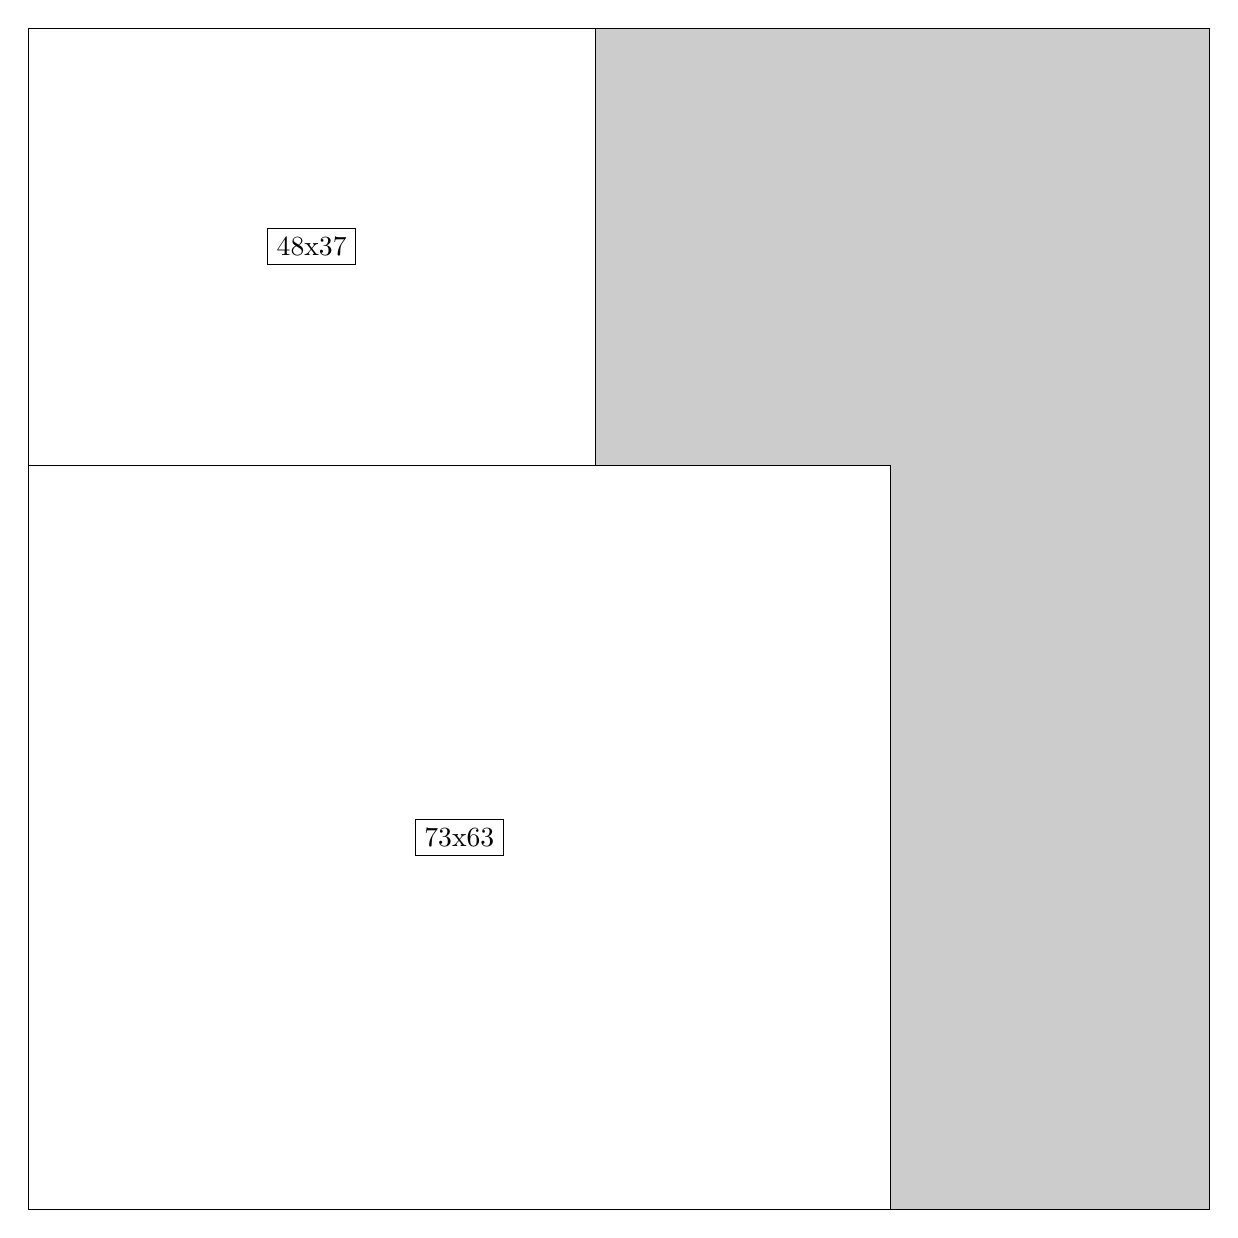
\begin{tikzpicture}[shorten >=1pt,scale=1.0,every node/.style={scale=1.0},->]
\tikzstyle{vertex}=[circle,fill=black!25,minimum size=14pt,inner sep=0pt]
\filldraw[fill=gray!40!white, draw=black] (0,0) rectangle (15.0,15.0);
\foreach \name/\x/\y/\w/\h in {73x63/0.0/0.0/10.95/9.45,48x37/0.0/9.45/7.199999999999999/5.55}
\filldraw[fill=white!40!white, draw=black] (\x,\y) rectangle node[draw] (\name) {\name} ++(\w,\h);
\end{tikzpicture}


w =73 , h =63 , x =0 , y =0 , v =4599
\par
w =48 , h =37 , x =0 , y =63 , v =1776
\par
\newpage


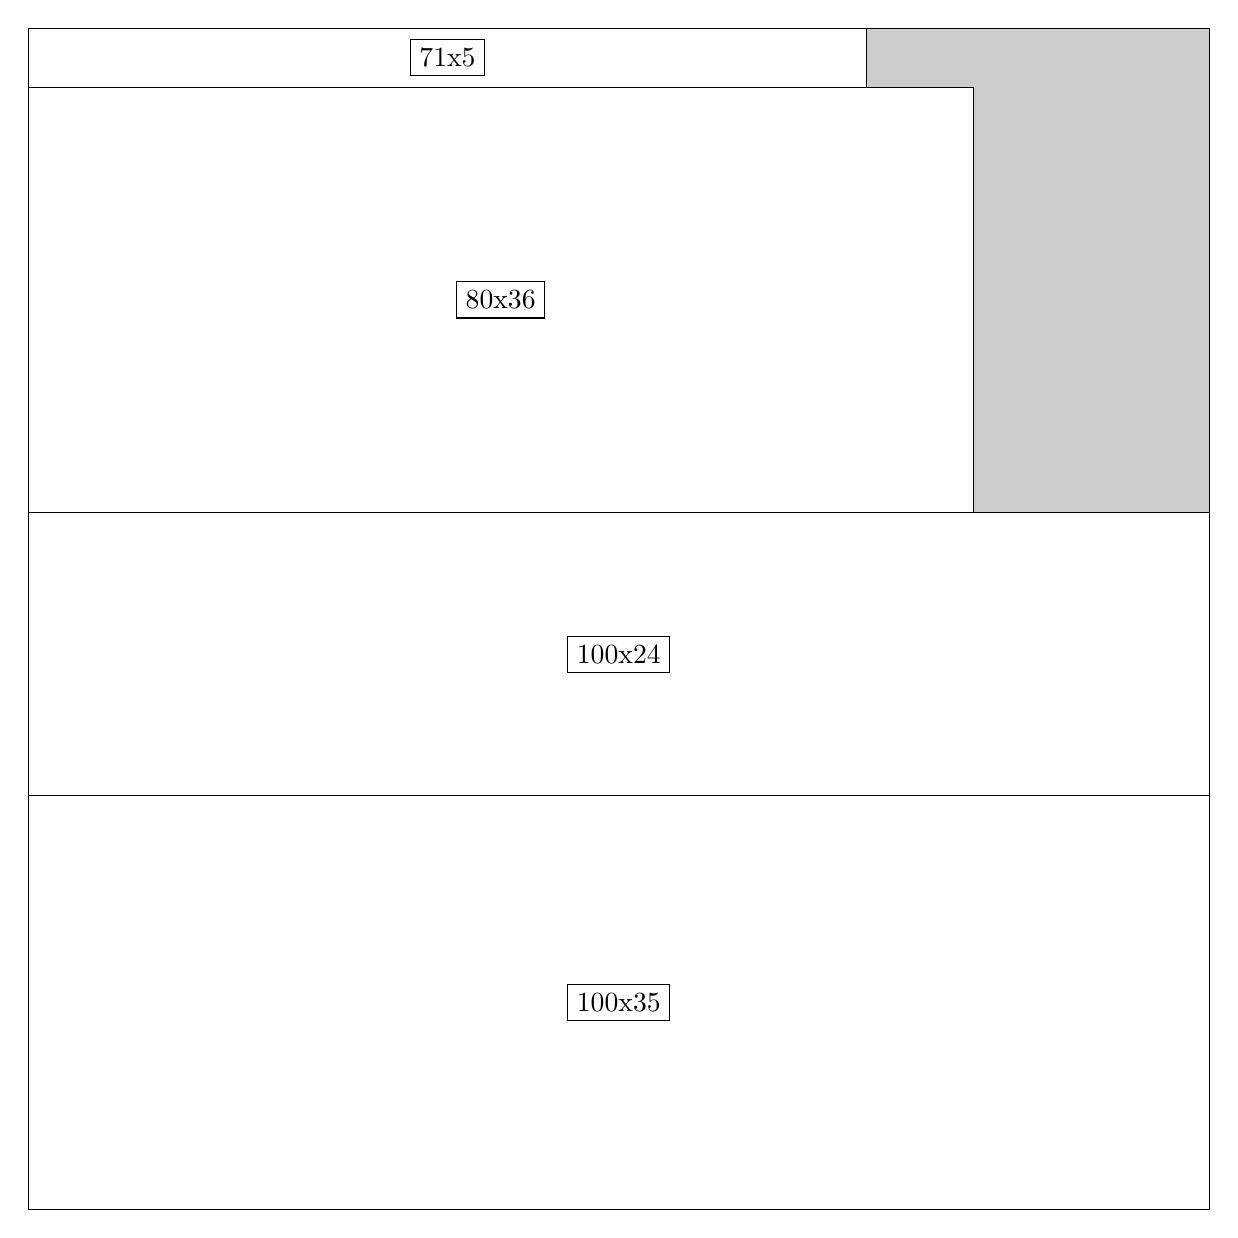
\begin{tikzpicture}[shorten >=1pt,scale=1.0,every node/.style={scale=1.0},->]
\tikzstyle{vertex}=[circle,fill=black!25,minimum size=14pt,inner sep=0pt]
\filldraw[fill=gray!40!white, draw=black] (0,0) rectangle (15.0,15.0);
\foreach \name/\x/\y/\w/\h in {100x35/0.0/0.0/15.0/5.25,80x36/0.0/8.85/12.0/5.3999999999999995,100x24/0.0/5.25/15.0/3.5999999999999996,71x5/0.0/14.25/10.65/0.75}
\filldraw[fill=white!40!white, draw=black] (\x,\y) rectangle node[draw] (\name) {\name} ++(\w,\h);
\end{tikzpicture}


w =100 , h =35 , x =0 , y =0 , v =3500
\par
w =80 , h =36 , x =0 , y =59 , v =2880
\par
w =100 , h =24 , x =0 , y =35 , v =2400
\par
w =71 , h =5 , x =0 , y =95 , v =355
\par
\newpage


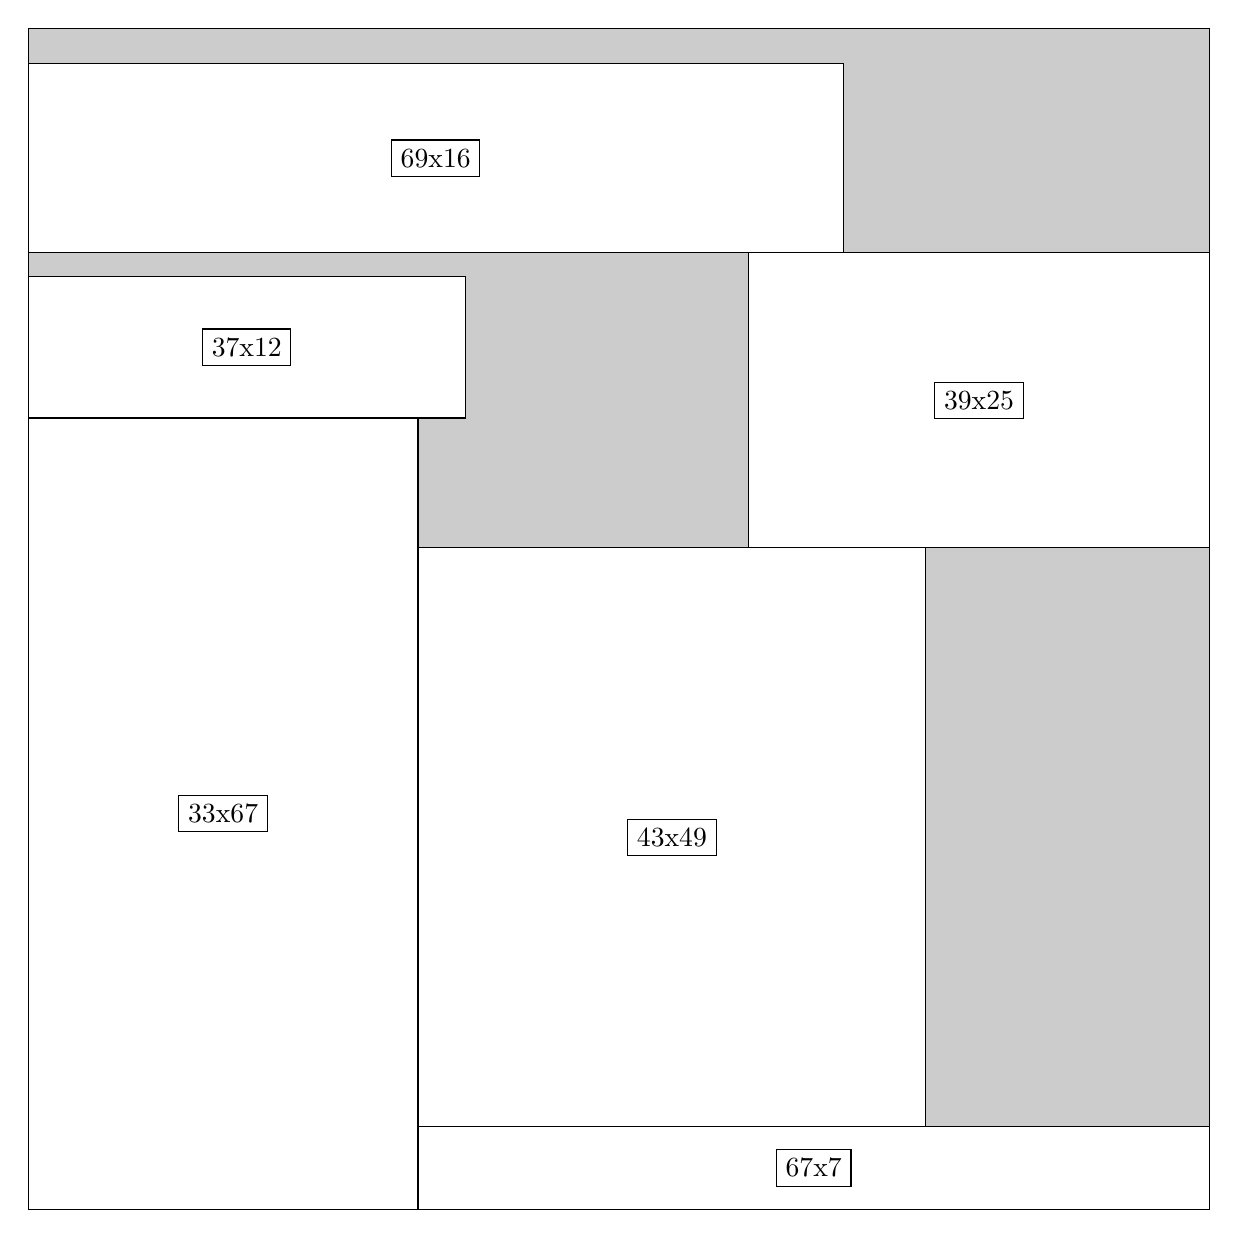
\begin{tikzpicture}[shorten >=1pt,scale=1.0,every node/.style={scale=1.0},->]
\tikzstyle{vertex}=[circle,fill=black!25,minimum size=14pt,inner sep=0pt]
\filldraw[fill=gray!40!white, draw=black] (0,0) rectangle (15.0,15.0);
\foreach \name/\x/\y/\w/\h in {33x67/0.0/0.0/4.95/10.049999999999999,43x49/4.95/1.05/6.45/7.35,69x16/0.0/12.15/10.35/2.4,39x25/9.15/8.4/5.85/3.75,67x7/4.95/0.0/10.049999999999999/1.05,37x12/0.0/10.049999999999999/5.55/1.7999999999999998}
\filldraw[fill=white!40!white, draw=black] (\x,\y) rectangle node[draw] (\name) {\name} ++(\w,\h);
\end{tikzpicture}


w =33 , h =67 , x =0 , y =0 , v =2211
\par
w =43 , h =49 , x =33 , y =7 , v =2107
\par
w =69 , h =16 , x =0 , y =81 , v =1104
\par
w =39 , h =25 , x =61 , y =56 , v =975
\par
w =67 , h =7 , x =33 , y =0 , v =469
\par
w =37 , h =12 , x =0 , y =67 , v =444
\par
\newpage


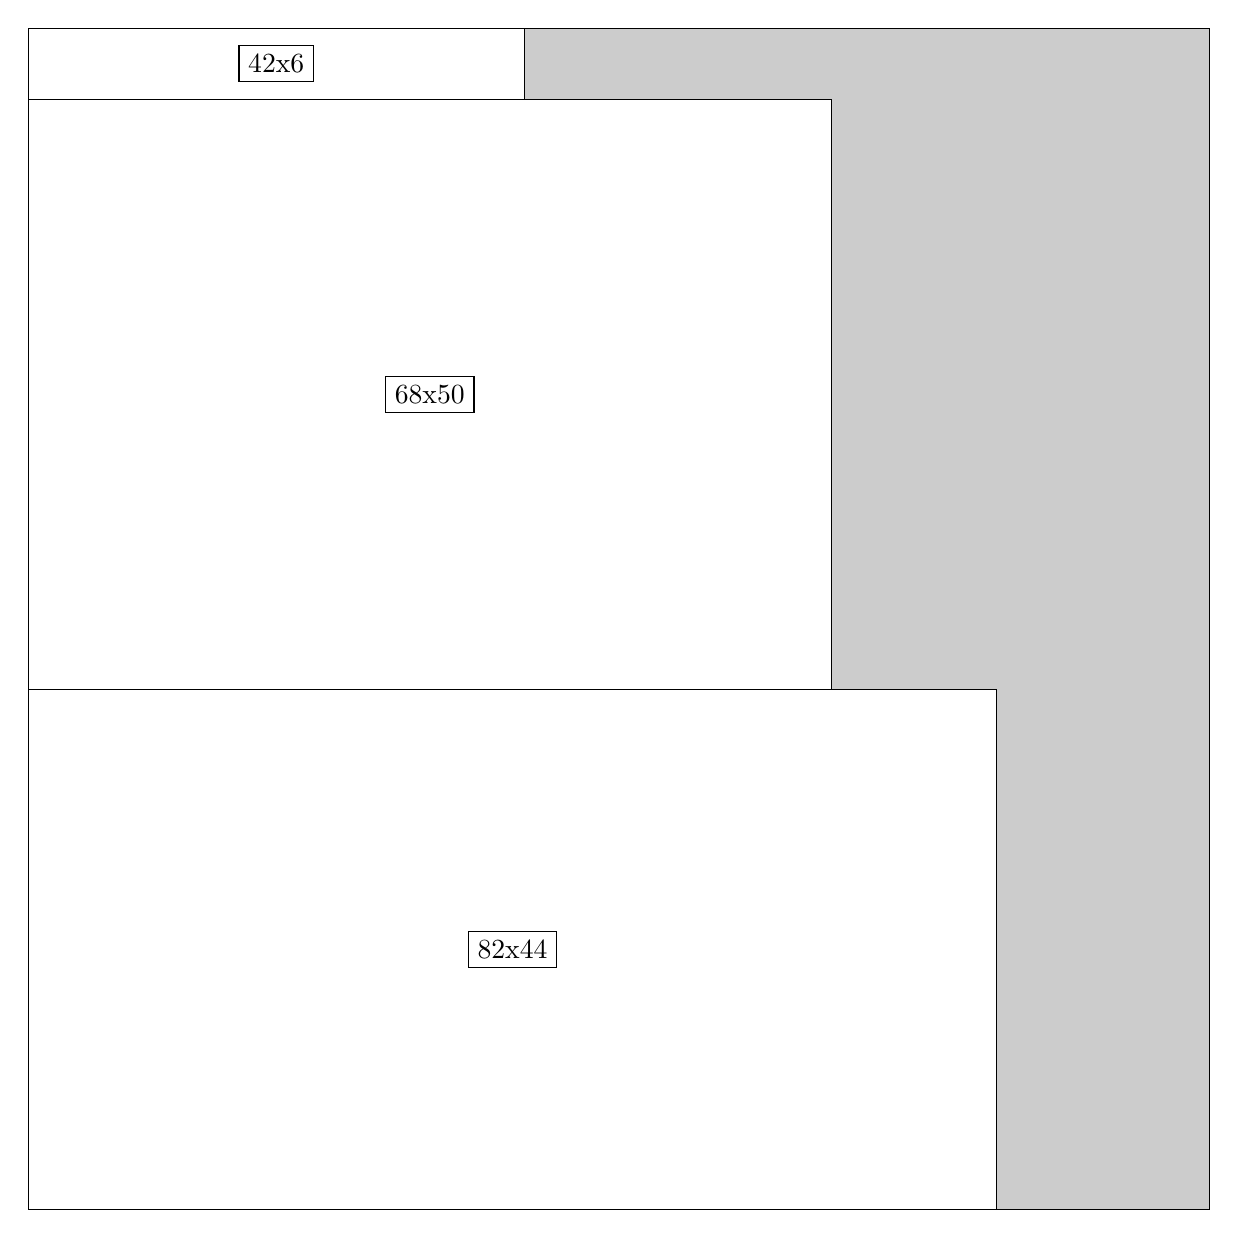
\begin{tikzpicture}[shorten >=1pt,scale=1.0,every node/.style={scale=1.0},->]
\tikzstyle{vertex}=[circle,fill=black!25,minimum size=14pt,inner sep=0pt]
\filldraw[fill=gray!40!white, draw=black] (0,0) rectangle (15.0,15.0);
\foreach \name/\x/\y/\w/\h in {82x44/0.0/0.0/12.299999999999999/6.6,68x50/0.0/6.6/10.2/7.5,42x6/0.0/14.1/6.3/0.8999999999999999}
\filldraw[fill=white!40!white, draw=black] (\x,\y) rectangle node[draw] (\name) {\name} ++(\w,\h);
\end{tikzpicture}


w =82 , h =44 , x =0 , y =0 , v =3608
\par
w =68 , h =50 , x =0 , y =44 , v =3400
\par
w =42 , h =6 , x =0 , y =94 , v =252
\par
\newpage


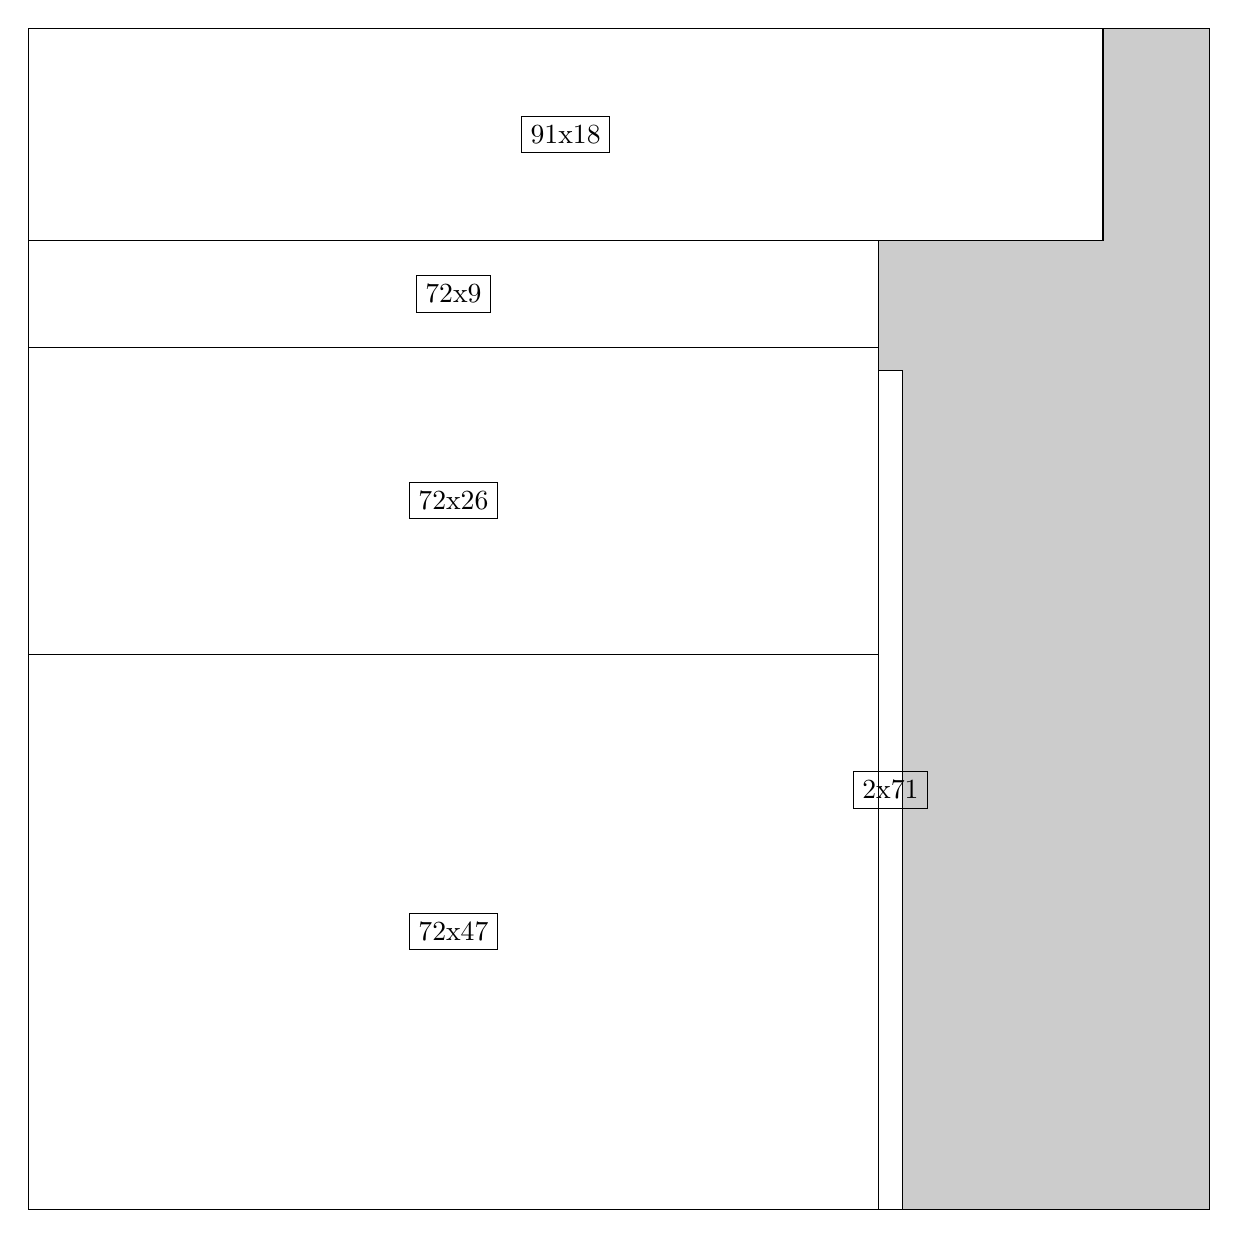
\begin{tikzpicture}[shorten >=1pt,scale=1.0,every node/.style={scale=1.0},->]
\tikzstyle{vertex}=[circle,fill=black!25,minimum size=14pt,inner sep=0pt]
\filldraw[fill=gray!40!white, draw=black] (0,0) rectangle (15.0,15.0);
\foreach \name/\x/\y/\w/\h in {72x47/0.0/0.0/10.799999999999999/7.05,72x26/0.0/7.05/10.799999999999999/3.9,91x18/0.0/12.299999999999999/13.65/2.6999999999999997,72x9/0.0/10.95/10.799999999999999/1.3499999999999999,2x71/10.799999999999999/0.0/0.3/10.65}
\filldraw[fill=white!40!white, draw=black] (\x,\y) rectangle node[draw] (\name) {\name} ++(\w,\h);
\end{tikzpicture}


w =72 , h =47 , x =0 , y =0 , v =3384
\par
w =72 , h =26 , x =0 , y =47 , v =1872
\par
w =91 , h =18 , x =0 , y =82 , v =1638
\par
w =72 , h =9 , x =0 , y =73 , v =648
\par
w =2 , h =71 , x =72 , y =0 , v =142
\par
\newpage


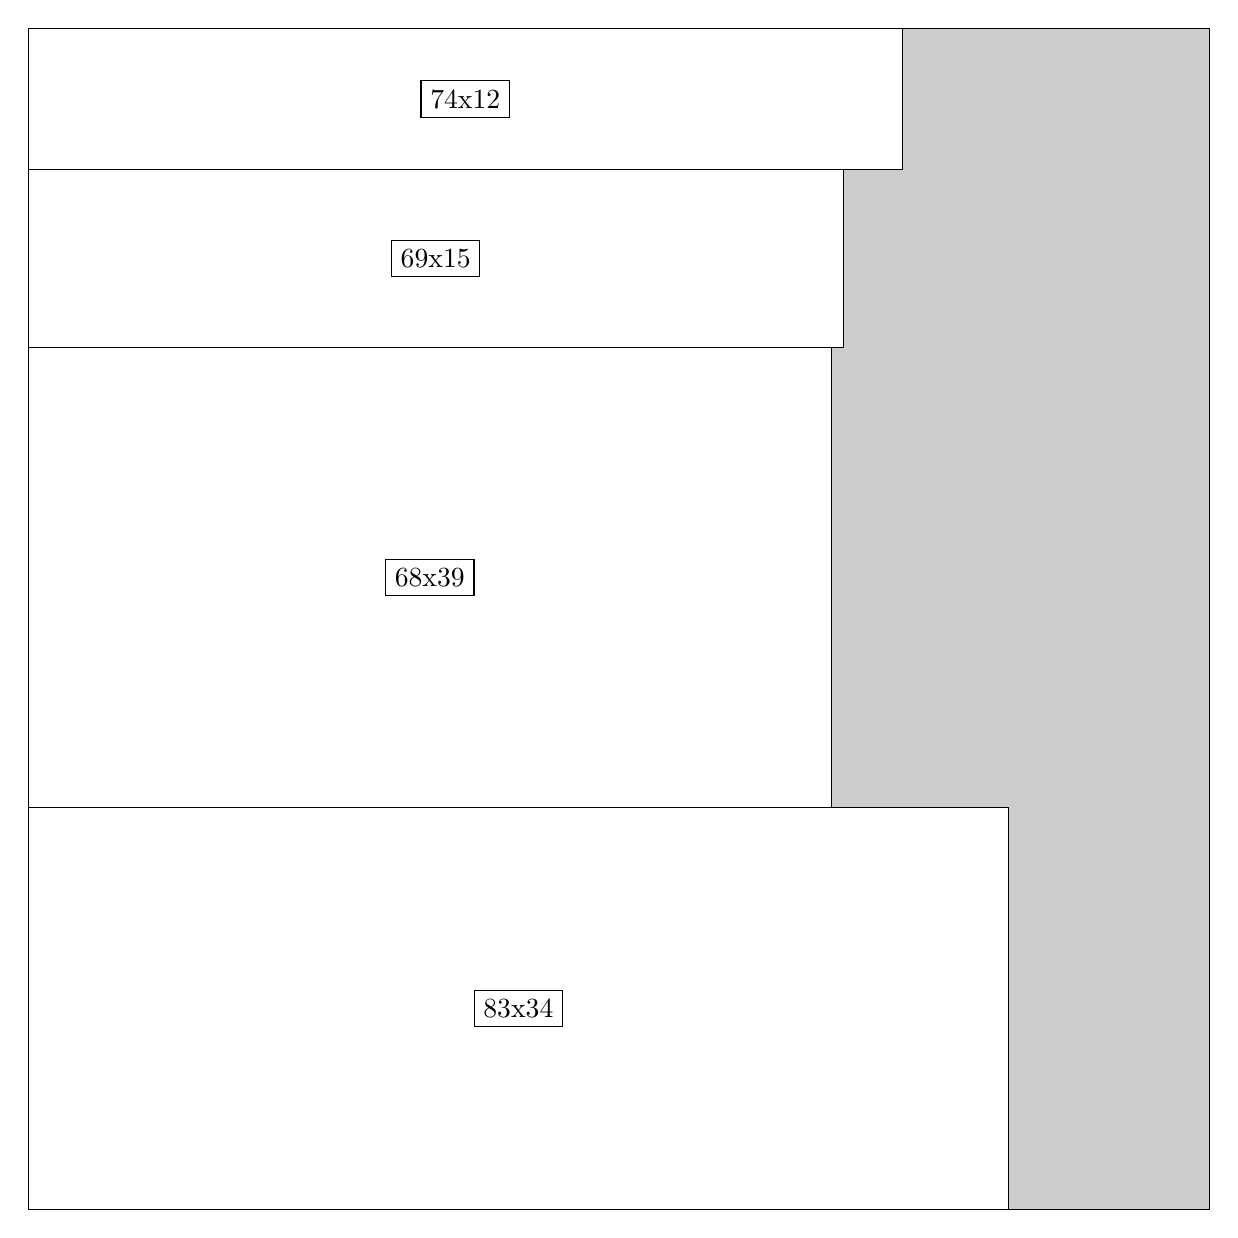
\begin{tikzpicture}[shorten >=1pt,scale=1.0,every node/.style={scale=1.0},->]
\tikzstyle{vertex}=[circle,fill=black!25,minimum size=14pt,inner sep=0pt]
\filldraw[fill=gray!40!white, draw=black] (0,0) rectangle (15.0,15.0);
\foreach \name/\x/\y/\w/\h in {83x34/0.0/0.0/12.45/5.1,68x39/0.0/5.1/10.2/5.85,69x15/0.0/10.95/10.35/2.25,74x12/0.0/13.2/11.1/1.7999999999999998}
\filldraw[fill=white!40!white, draw=black] (\x,\y) rectangle node[draw] (\name) {\name} ++(\w,\h);
\end{tikzpicture}


w =83 , h =34 , x =0 , y =0 , v =2822
\par
w =68 , h =39 , x =0 , y =34 , v =2652
\par
w =69 , h =15 , x =0 , y =73 , v =1035
\par
w =74 , h =12 , x =0 , y =88 , v =888
\par
\newpage


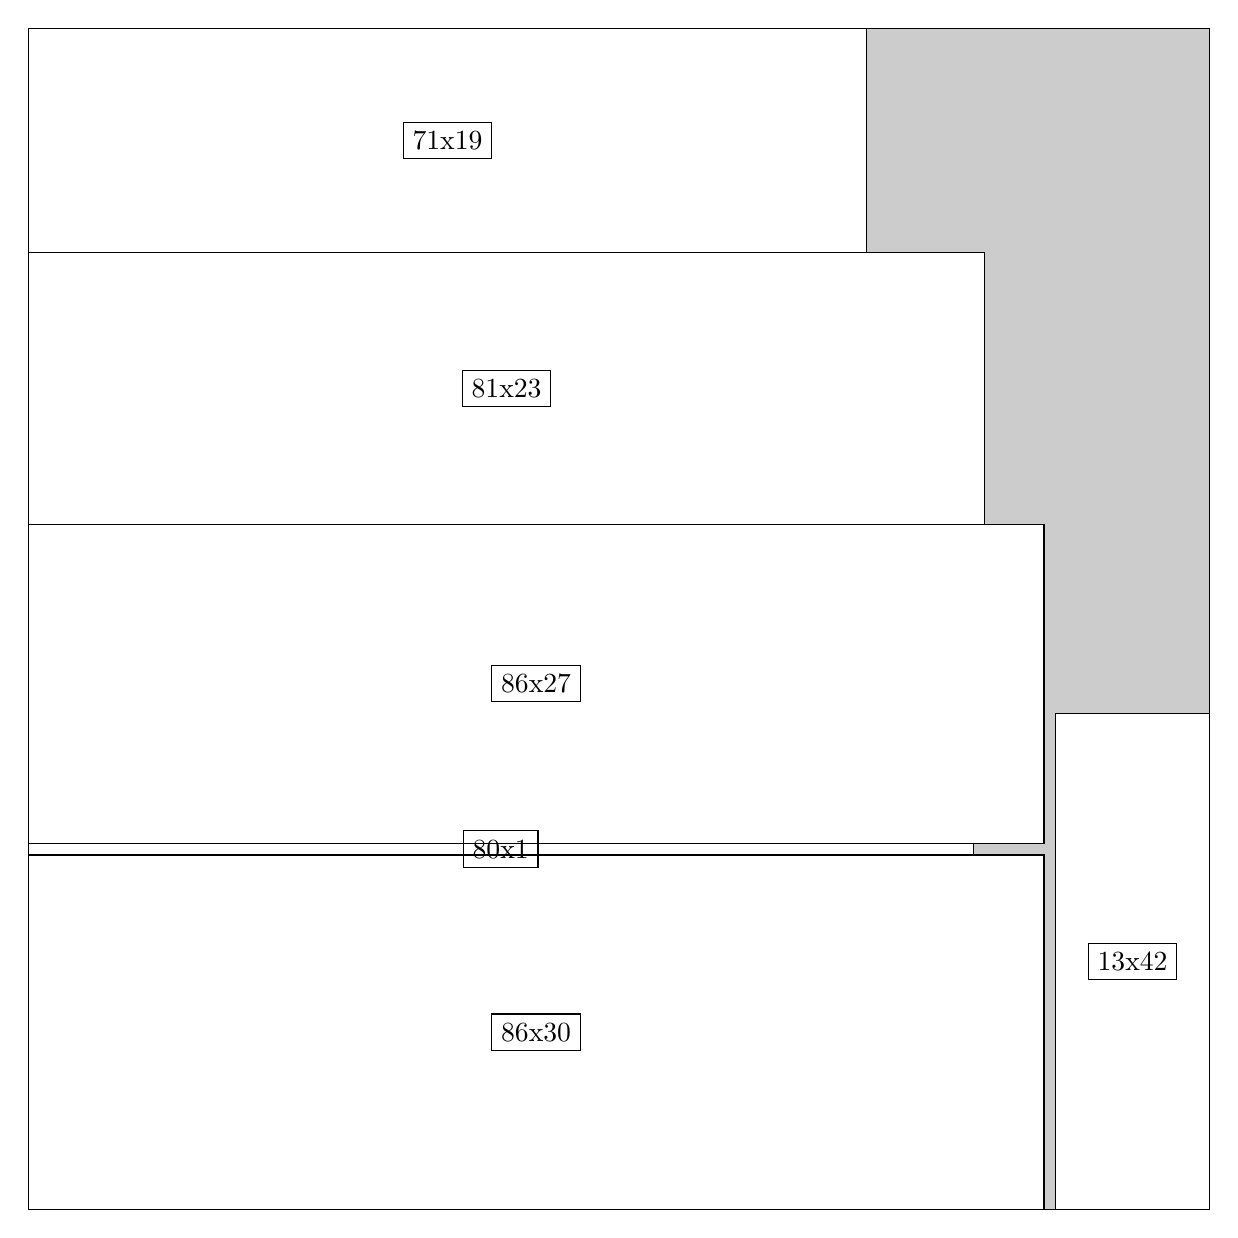
\begin{tikzpicture}[shorten >=1pt,scale=1.0,every node/.style={scale=1.0},->]
\tikzstyle{vertex}=[circle,fill=black!25,minimum size=14pt,inner sep=0pt]
\filldraw[fill=gray!40!white, draw=black] (0,0) rectangle (15.0,15.0);
\foreach \name/\x/\y/\w/\h in {86x30/0.0/0.0/12.9/4.5,86x27/0.0/4.6499999999999995/12.9/4.05,81x23/0.0/8.7/12.15/3.4499999999999997,71x19/0.0/12.15/10.65/2.85,13x42/13.049999999999999/0.0/1.95/6.3,80x1/0.0/4.5/12.0/0.15}
\filldraw[fill=white!40!white, draw=black] (\x,\y) rectangle node[draw] (\name) {\name} ++(\w,\h);
\end{tikzpicture}


w =86 , h =30 , x =0 , y =0 , v =2580
\par
w =86 , h =27 , x =0 , y =31 , v =2322
\par
w =81 , h =23 , x =0 , y =58 , v =1863
\par
w =71 , h =19 , x =0 , y =81 , v =1349
\par
w =13 , h =42 , x =87 , y =0 , v =546
\par
w =80 , h =1 , x =0 , y =30 , v =80
\par
\newpage


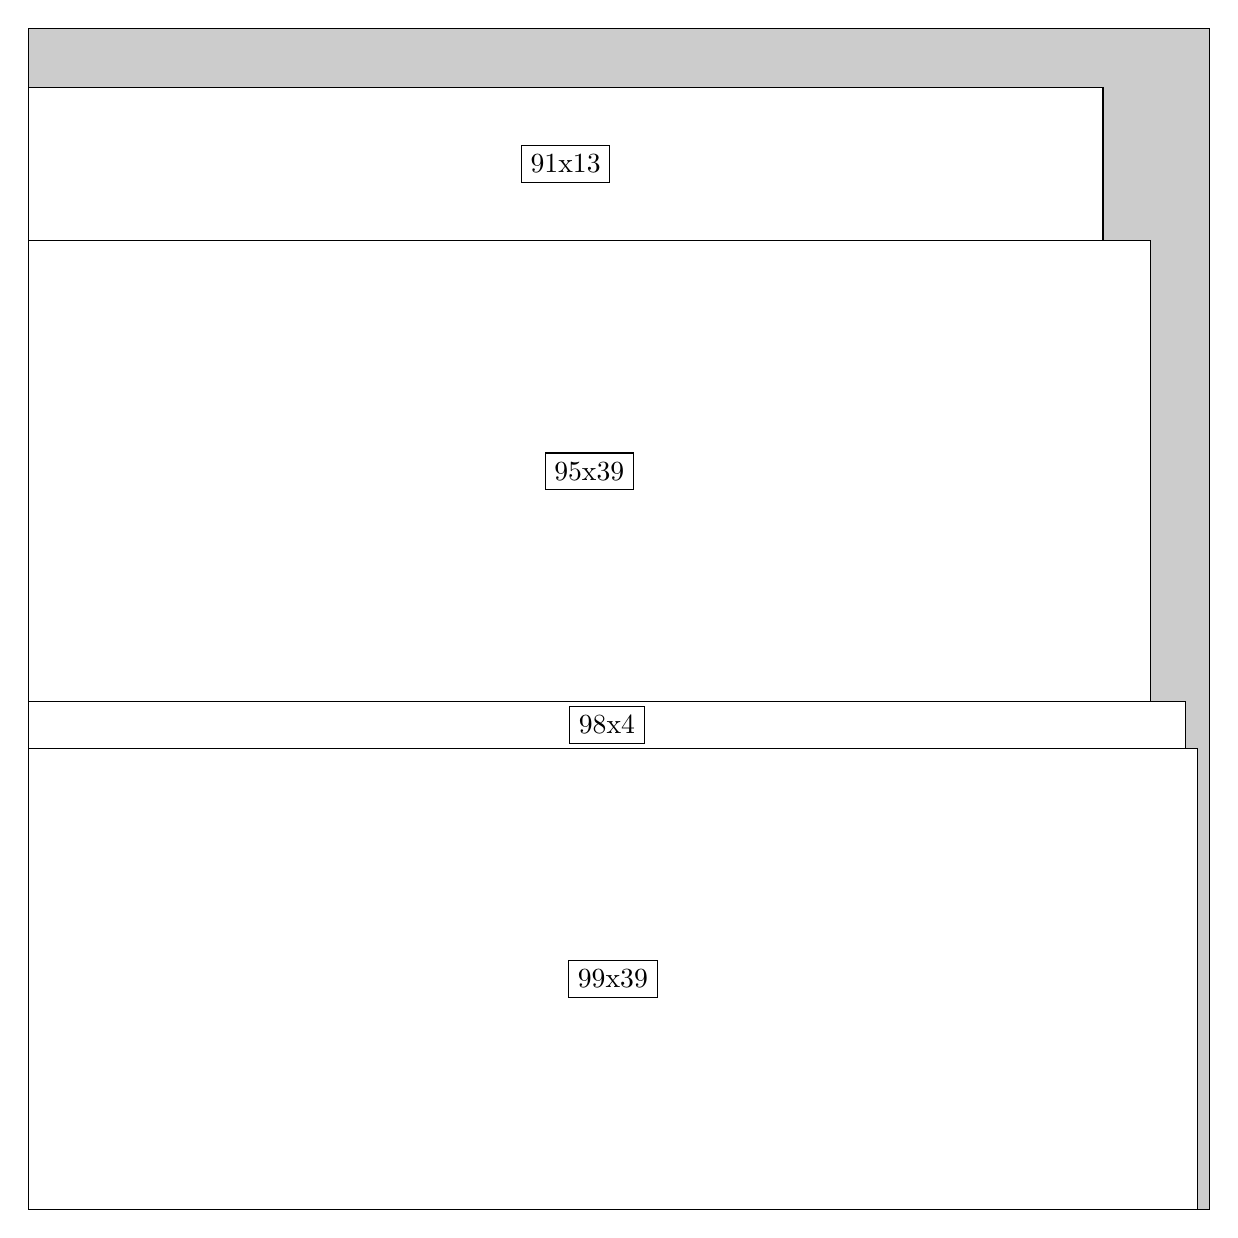
\begin{tikzpicture}[shorten >=1pt,scale=1.0,every node/.style={scale=1.0},->]
\tikzstyle{vertex}=[circle,fill=black!25,minimum size=14pt,inner sep=0pt]
\filldraw[fill=gray!40!white, draw=black] (0,0) rectangle (15.0,15.0);
\foreach \name/\x/\y/\w/\h in {99x39/0.0/0.0/14.85/5.85,95x39/0.0/6.45/14.25/5.85,91x13/0.0/12.299999999999999/13.65/1.95,98x4/0.0/5.85/14.7/0.6}
\filldraw[fill=white!40!white, draw=black] (\x,\y) rectangle node[draw] (\name) {\name} ++(\w,\h);
\end{tikzpicture}


w =99 , h =39 , x =0 , y =0 , v =3861
\par
w =95 , h =39 , x =0 , y =43 , v =3705
\par
w =91 , h =13 , x =0 , y =82 , v =1183
\par
w =98 , h =4 , x =0 , y =39 , v =392
\par
\newpage


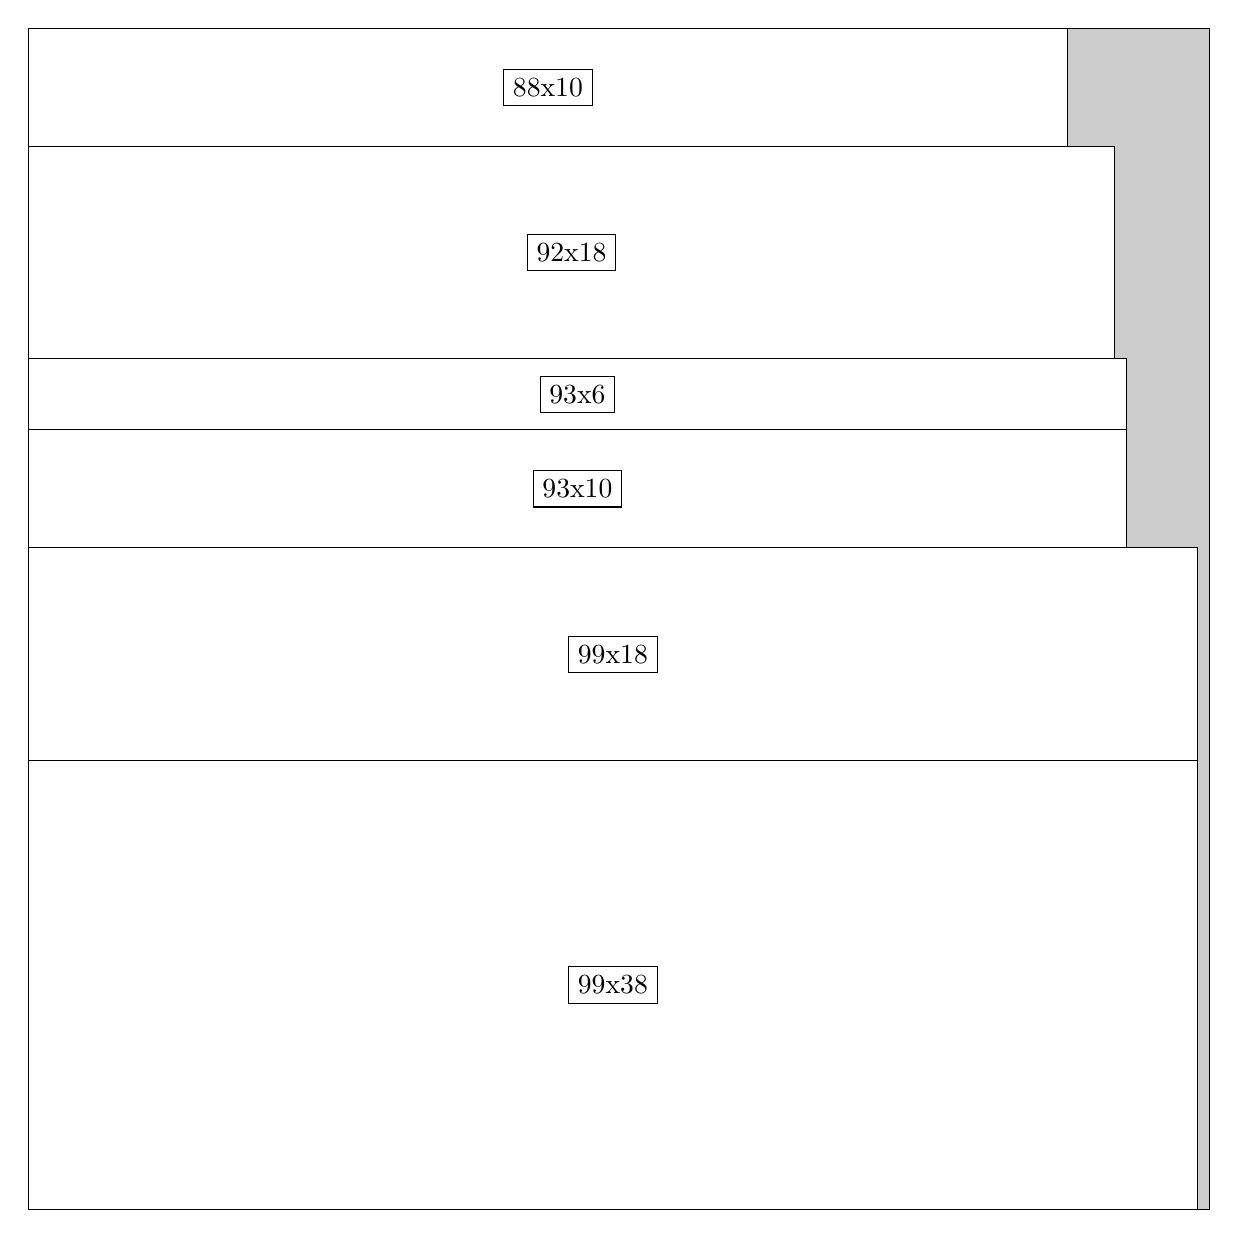
\begin{tikzpicture}[shorten >=1pt,scale=1.0,every node/.style={scale=1.0},->]
\tikzstyle{vertex}=[circle,fill=black!25,minimum size=14pt,inner sep=0pt]
\filldraw[fill=gray!40!white, draw=black] (0,0) rectangle (15.0,15.0);
\foreach \name/\x/\y/\w/\h in {99x38/0.0/0.0/14.85/5.7,99x18/0.0/5.7/14.85/2.6999999999999997,92x18/0.0/10.799999999999999/13.799999999999999/2.6999999999999997,93x10/0.0/8.4/13.95/1.5,88x10/0.0/13.5/13.2/1.5,93x6/0.0/9.9/13.95/0.8999999999999999}
\filldraw[fill=white!40!white, draw=black] (\x,\y) rectangle node[draw] (\name) {\name} ++(\w,\h);
\end{tikzpicture}


w =99 , h =38 , x =0 , y =0 , v =3762
\par
w =99 , h =18 , x =0 , y =38 , v =1782
\par
w =92 , h =18 , x =0 , y =72 , v =1656
\par
w =93 , h =10 , x =0 , y =56 , v =930
\par
w =88 , h =10 , x =0 , y =90 , v =880
\par
w =93 , h =6 , x =0 , y =66 , v =558
\par
\newpage


\end{document}